\documentclass[a4paper,11pt]{article}
\usepackage[T1]{fontenc}
\usepackage[utf8]{inputenc}
\usepackage[italian]{babel}
\usepackage{csquotes}

%\usepackage[rightcaption]{sidecap}
\usepackage{hyperref}
\usepackage{graphicx}
\usepackage{subcaption}
\graphicspath{{./images}}

\usepackage{biblatex}
\addbibresource{material.bib} %Import the bibliography file

\usepackage{amssymb}
\usepackage{physics}

\begin{document}
    \author{Federico Forzano}
    \title{Valutazione prestazioni in comunicazioni PASS}
    \maketitle

    \section{Prestazioni \foreignlanguage{english}{Photon Added Coherent States}}
        \subsection{Riproduzione dei risultati}
        Il primo obiettivo ottenuto è stato riprodurre i risultati 
        riguardanti le prestazioni di un sistema PACS.

        A partire dalla rappresentazione nella base di Fock, dello stato noisy PACS 
        $\Xi(\mu,k)$ (con $\mu$ ampiezza dello stato coerente di partenza e $k$ numero di 
        fotoni aggiunti):
        \begin{equation}
            \bra{n}\Xi(\mu,k)\ket{m}=
            \begin{cases}
                c_{n,m}^{(k)}\ se\ n,m\geqslant0\\
                0\ altrimenti
            \end{cases}
        \end{equation}
        con
        \begin{equation}
            c_{n,m}^{(k)}=\frac{(1-v)^{k+1}e^{-(1-v)\absolutevalue{\mu}^{2}}}
            {v^k}\sqrt{\frac{n!}{m!}}\binom{n}{k}v^n[(1-v)\mu^*]^{m-n}
            \frac{L_{n-k}^{m-n}(\frac{-(1-v)^2\absolutevalue{\mu}^{2}}{v})}{L_k(-(1-v)\absolutevalue{\mu}^{2})}
        \end{equation}

        è possibile calcolare la probabilità di errore la probabilità di errore (DEP)
        nel caso di discriminatore ottimo (MDEP), grazie all'espressione (Helstrom Bound):
        \begin{equation}
            \hat{Pe}=\frac{1}{2}(1-\norm{p_1\Xi_1-p_0\Xi_0}_1).
            \label{eq:3}
        \end{equation}

        \begin{figure}[ht]
            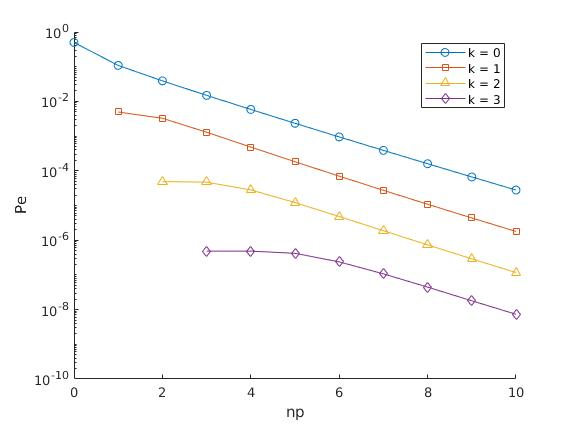
\includegraphics[width=1\textwidth]{4a.jpg}
            \caption{Performance of QSD between a noisy PACS and the thermal 
            state as a function of np, with $\bar{n}$, $p0=p1=1/2$}
            \label{fig:1}
        \end{figure}

        In figura \ref{fig:1} si può osservare l'effetto della \foreignlanguage{english}
        {photon addition} per la MDEP in funzione del numero di fotoni nel sistema
        ($n_p$), con $\bar{n}=10^{-2}$ e $p_0=p_1=1/2$.
        (L'inversione della funzione che a $\mu$ e $k$ associa $n_p$ è realizzata tramite 
        un algoritmo di bisezione numerica con errore di approssimazione $\delta=10^{-6}$).

        \subsection{Valutazione dell'effetto del rumore termico}
        Nel caso di rumore termico nullo ($\bar{n}=0$), l'espressione per il calcolo della
        MDEP \ref{eq:3} diventa:
        \begin{equation}
            \hat{Pe}=\frac{1}{2}(1-4 p_0 p_1\absolutevalue{\braket{\psi_0}{\psi_1}}^2)
        \end{equation}
        con 
        $\ket{\psi_0}=\ket{\xi^{(h)}}$,
        $\ket{\psi_0}=\ket{\mu^{(h)}}$
        e il prodotto scalare dato in forma esplicita da:
        \begin{equation}
            \braket{\xi^{(h)}}{\mu^{(h)}}=\frac{(\xi^*)^{k-h}L_h^{k-h}(-\mu\xi^*)
            e^{-1/2(\absolutevalue{\mu}^2+\absolutevalue{\xi}^2-2\mu\xi^*)}}
            {\sqrt{\frac{k!}{h!}L_k(-\absolutevalue{\mu^2})L_h(-\absolutevalue{\xi}^2)}}
        \end{equation}.

        È possibile individuare quindi, alcuni zeri della MDEP per $\xi=0$ e per $L_h^{k-h}(-\mu\xi^*)=0$. 
        In corrispondenza di quest'ultimi, si è studiato l'effetto del rumore termico.
        
        \begin{figure}[ht]
            \caption{MDEP without noise}
            \begin{subfigure}{0.49\textwidth}
                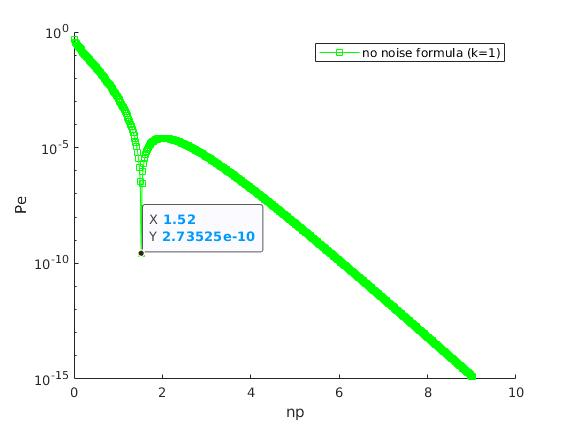
\includegraphics[width=\linewidth]{k1LaguerreZeros.jpg}
                \caption{$k=1$}
            \end{subfigure}
            \hspace*{\fill}
            \begin{subfigure}{0.49\textwidth}
                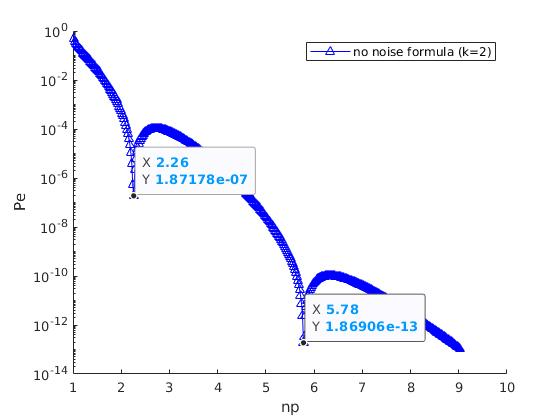
\includegraphics[width=\linewidth]{k2LaguerreZeros.jpg}
                \caption{$k=2$}
            \end{subfigure}
            \label{fig:2}
        \end{figure}
        \begin{figure}[ht]
            \caption{Effetto del rumore termico}
            \begin{subfigure}{0.45\textwidth}
                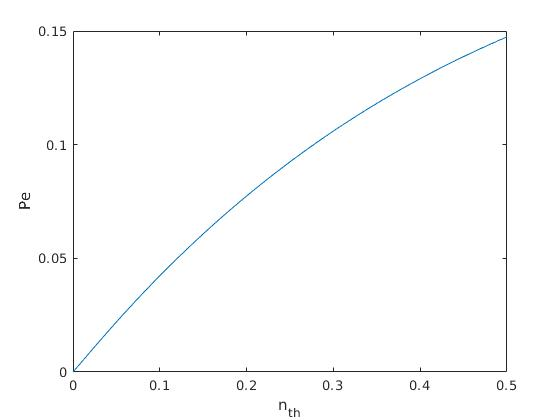
\includegraphics[width=\linewidth]{noiseEffectk1.jpg}
                \caption{$k=1$, $\mu=0.54$}
            \end{subfigure}
            \hspace*{\fill}
            \begin{subfigure}{0.45\textwidth}
                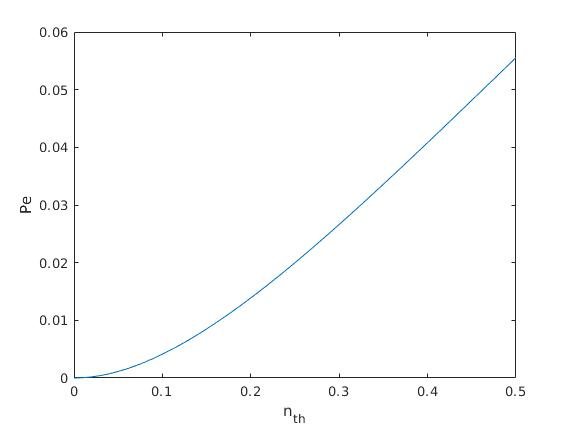
\includegraphics[width=\linewidth]{noiseEffectk2_zero2.jpg}
                \caption{$k=2$, $\mu=1.58$}
            \end{subfigure}
            \label{fig:3}
        \end{figure}

        Fissato $k$, si è studiato numericamente il valore degli zeri della MDEP in assenza di rumore
        \ref{fig:2}. Per questi valori di $\mu$ si è valutato l'effetto del rumore termico \ref{fig:3}.
        
        \subsection{Valutazione di un sistema PACS BPSK}
        I risultati precedentemente visti si riferiscono ad un sistema in cui:
        \equation{\Xi_0=\Xi_{th}(0)}$$
        \equation{\Xi_1=\Xi_{th}^{(k)}(\mu)}$$
        ovvero ad un sistema OOK quantistico con stati \foreignlanguage{english}{Photon Added}.

        \begin{figure}[ht]
            \caption{Confronto tra sistemi BPSK e OOK, per $k=0,1,2,3$}
            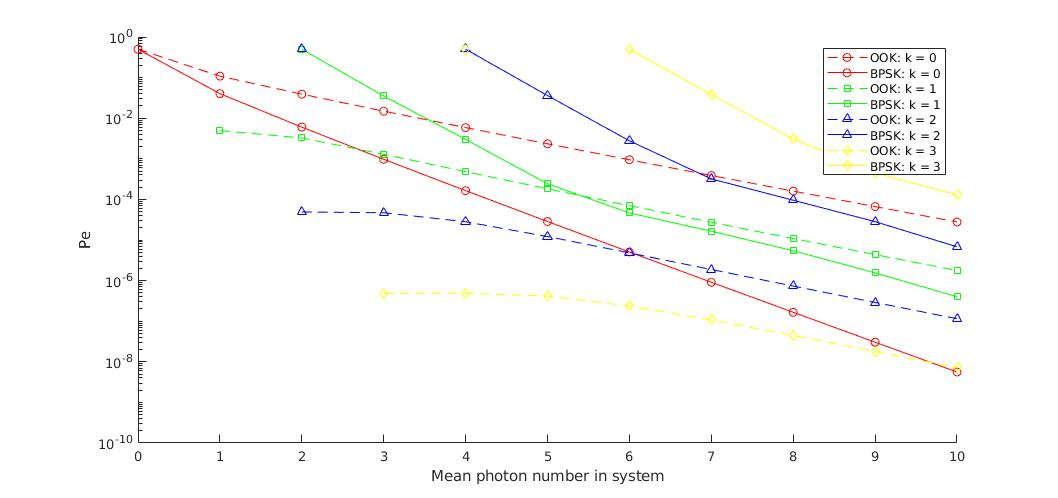
\includegraphics[width=\linewidth]{BPSK_comparison.jpg}
            \label{fig:4}
        \end{figure}

        Si è voluto testare le prestazioni di un sistema BPSK con stati \foreignlanguage{english}
        {Photon Added} \ref{fig:4}
        \equation{\Xi_0=\Xi_{th}^{(k)}(-\mu)}$$
        \equation{\Xi_1=\Xi_{th}^{(k)}(\mu)}.$$
        
    \section{Prestazioni \foreignlanguage{english}{Photon Added Squeezed States}}
    Per ovviare ai limiti intrinsechi nell'utilizzo di stati coerenti, si è pensato
    di utilizzare stati \foreignlanguage{english}{squeezed}, ovvero definiti come:
    \equation{\Xi_{th}(\mu,\zeta)=D(\mu)S(\zeta)\Xi_{th}S^\dagger(\zeta)D^\dagger(\mu)}$$
    con $\zeta=r e^{i\theta}$.
    Si sono dunque valutate le prestazioni di sistemi di comunicazione basati su questa tipologia
    di stati quantistici.

    \subsection{Sistemi \foreignlanguage{english}{noisy Squeezed States}}
    
    \begin{figure}[ht]
        \caption{\foreignlanguage{english}{Squeezed} BPSK, $\theta=\pi$, $p_0=p_1=\frac{1}{2}$}

        \begin{subfigure}{0.49\textwidth}
            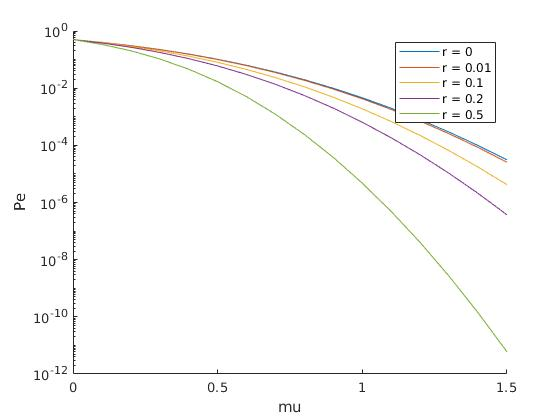
\includegraphics[width=\linewidth]{SSBPSK.jpg}
            \caption{$\bar{n}=0$}
        \end{subfigure}
        \hspace*{\fill}
        \begin{subfigure}{0.49\textwidth}
            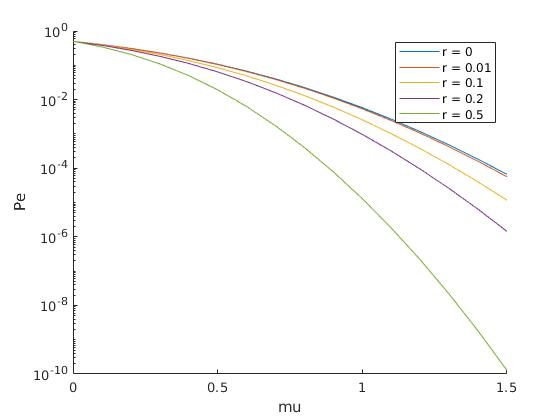
\includegraphics[width=\linewidth]{SSBPSKNoisy.jpg}
            \caption{$\bar{n}=10^{-2}$}
        \end{subfigure}
        \label{fig:5}
    \end{figure}

    In primo luogo si è voluto studiare l'effetto dello \foreignlanguage{english}
    {squeezing} senza \foreignlanguage{english}{photon addiction}, al variare di $r$, fissato 
    $\theta=\pi$. \ref{fig:5}
    Risulta evidente come, al variare di $r$, si ottenga un miglioramento delle prestazioni del sistema.

    \subsection{Sistemi \foreignlanguage{english}{noisy Photon Added Squeezed States}}
    \begin{figure}[ht]
        \caption{Confronto MDEP per BPSK PASS, $\bar{n}=10^{-2}$, $p_0=p_1=\frac{1}{2}$}
        %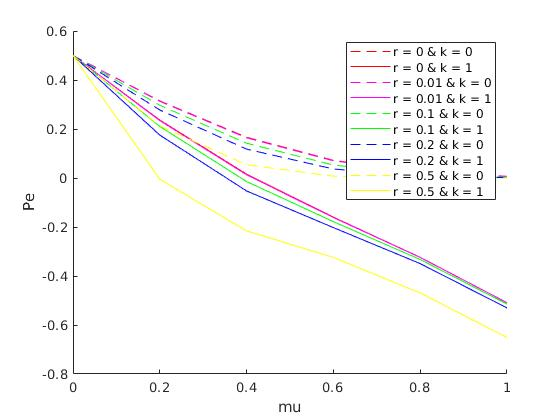
\includegraphics[width=\linewidth]{PASSBPSK.jpg}
        \label{fig:6}
    \end{figure}
    Si sono valutate dunque le prestazioni per sistemi \foreignlanguage{english}
    {photon added squeezed states}. \ref{fig:6}
    La \foreignlanguage{english}{density matrix} dello stato è ottenuta, a partire da quella per lo
    stato non \foreignlanguage{english}{photon added}, tramite:
    \begin{equation}
        \bra{n}\Xi_{th}^{(k)}(\mu,\zeta)\ket{m}=
            \begin{cases}
                0\ se\ n<k \lor m<k\\
                \sqrt{\frac{n!m!}{(n-k)!(m-k)!}}\bra{n-k}\Xi_{th}(\mu,\zeta)\ket{m-k}\ altrimenti
            \end{cases}
    \end{equation}
\end{document}

